
\section{Waterway Monitoring Example\marginnote{(Path Plannning and Assignment Message Flow Example)}}
In order to explain how UxAS uses LMCP messages to generate path plans and assign Unmanned Air Vehicles (UAV) to perform tasks, a waterway monitoring scenario has been constructed. In this example, the challenge is to generate the commands required to cause one of two UAVs to fly alongside and record imagery of a given section of the waterway. Figure \ref{fig:waterway} shows the waterway of interest, as well as the initial position of the two UAVs. Here are the rules for this scenario:
\graphicspath{{./figures/}}
\begin{marginfigure}
	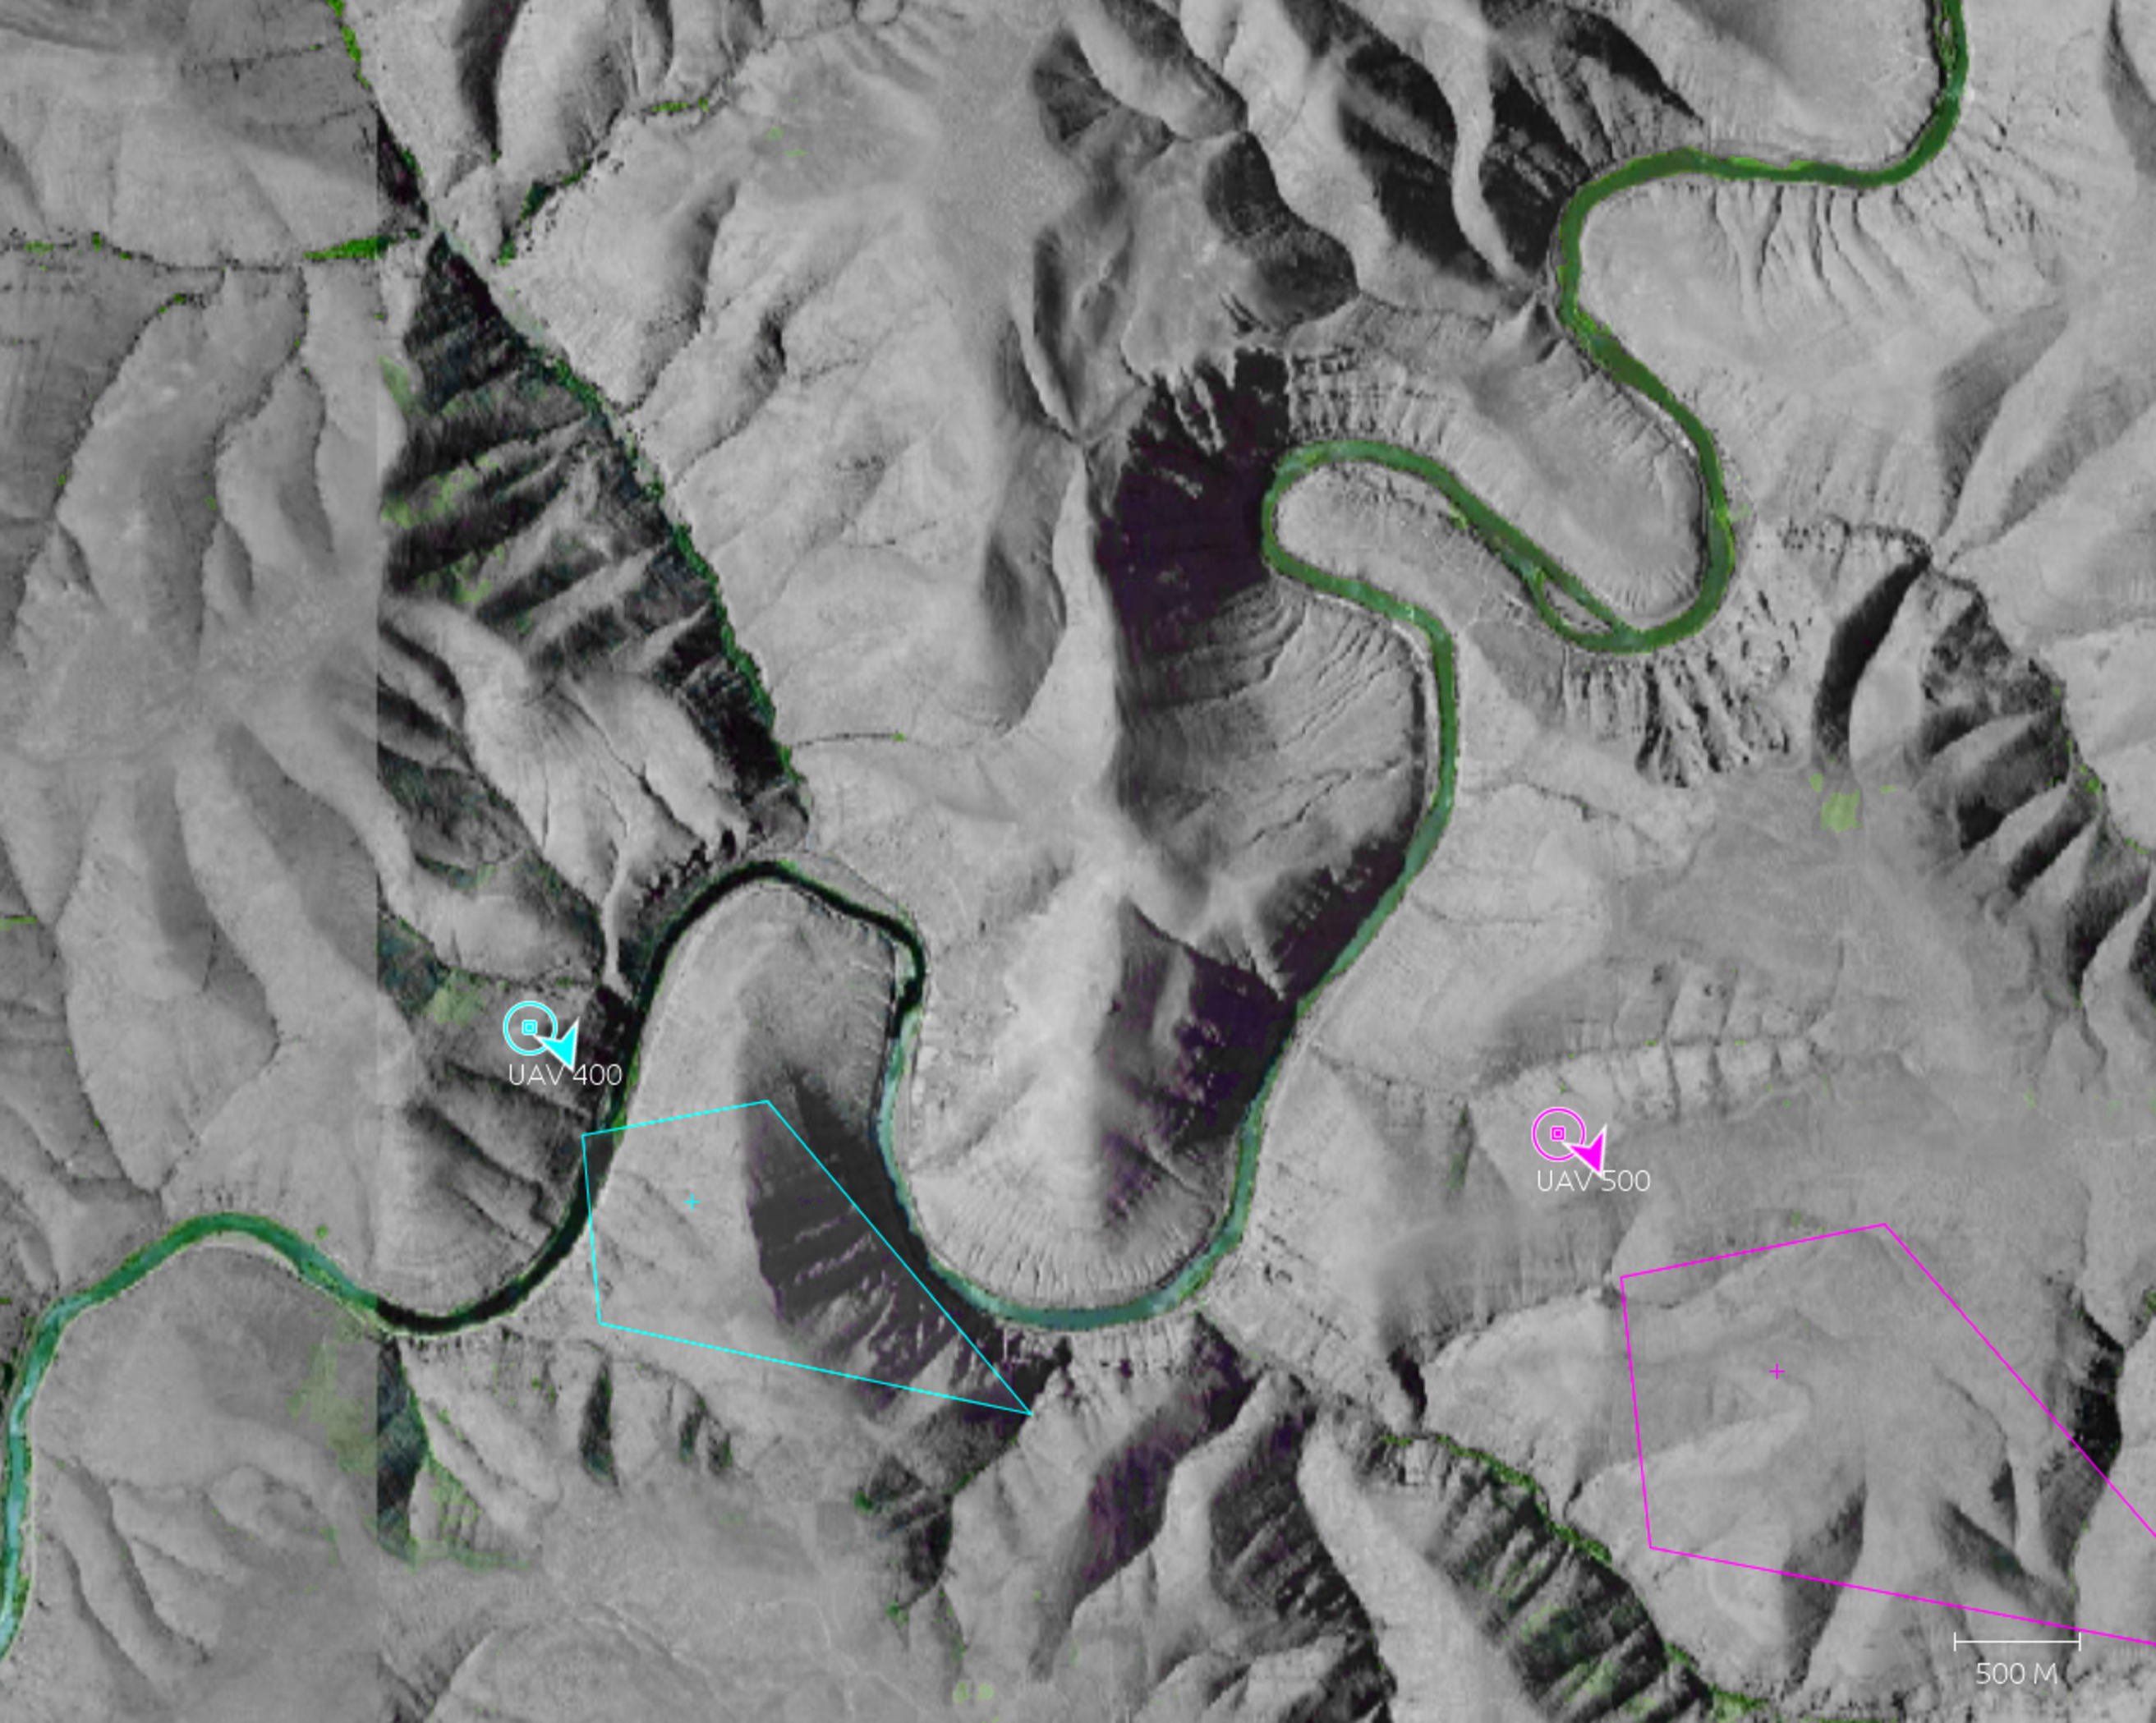
\includegraphics[width=1.3\linewidth]{\FiguresPath//01_WaterwaySearch_Initial}
	\caption{The waterway to be monitored.}
	\label{fig:waterway}
\end{marginfigure}

\begin{itemize}
	\item The plans/assignments are generated by UxAS on the ground. 
	\item A ground control station manages the message traffic between UxAS and the UAVs.
	\item The UAVs can start monitoring from either end of a waterway section.
	\item Each waterway section is to be monitored only one time.
	\item The UAVs must fly alongside the waterway section so that the sensor angle with respect to the waterway does not change
	\item The path plan/assignment should seek to minimize the maximum distance traveled by either of the UAVs.
\end{itemize}

\noindent Figure \ref{fig:MessageFlow_all} depicts the flow of messages between services required to create plans, assign a UAV, and point the UAV's sensor as the plans are being executed. This figure will be used as a guide to explain how UxAS uses messages to plan and implement the waterway monitoring scenario. 
\begin{marginfigure}[30pt]
	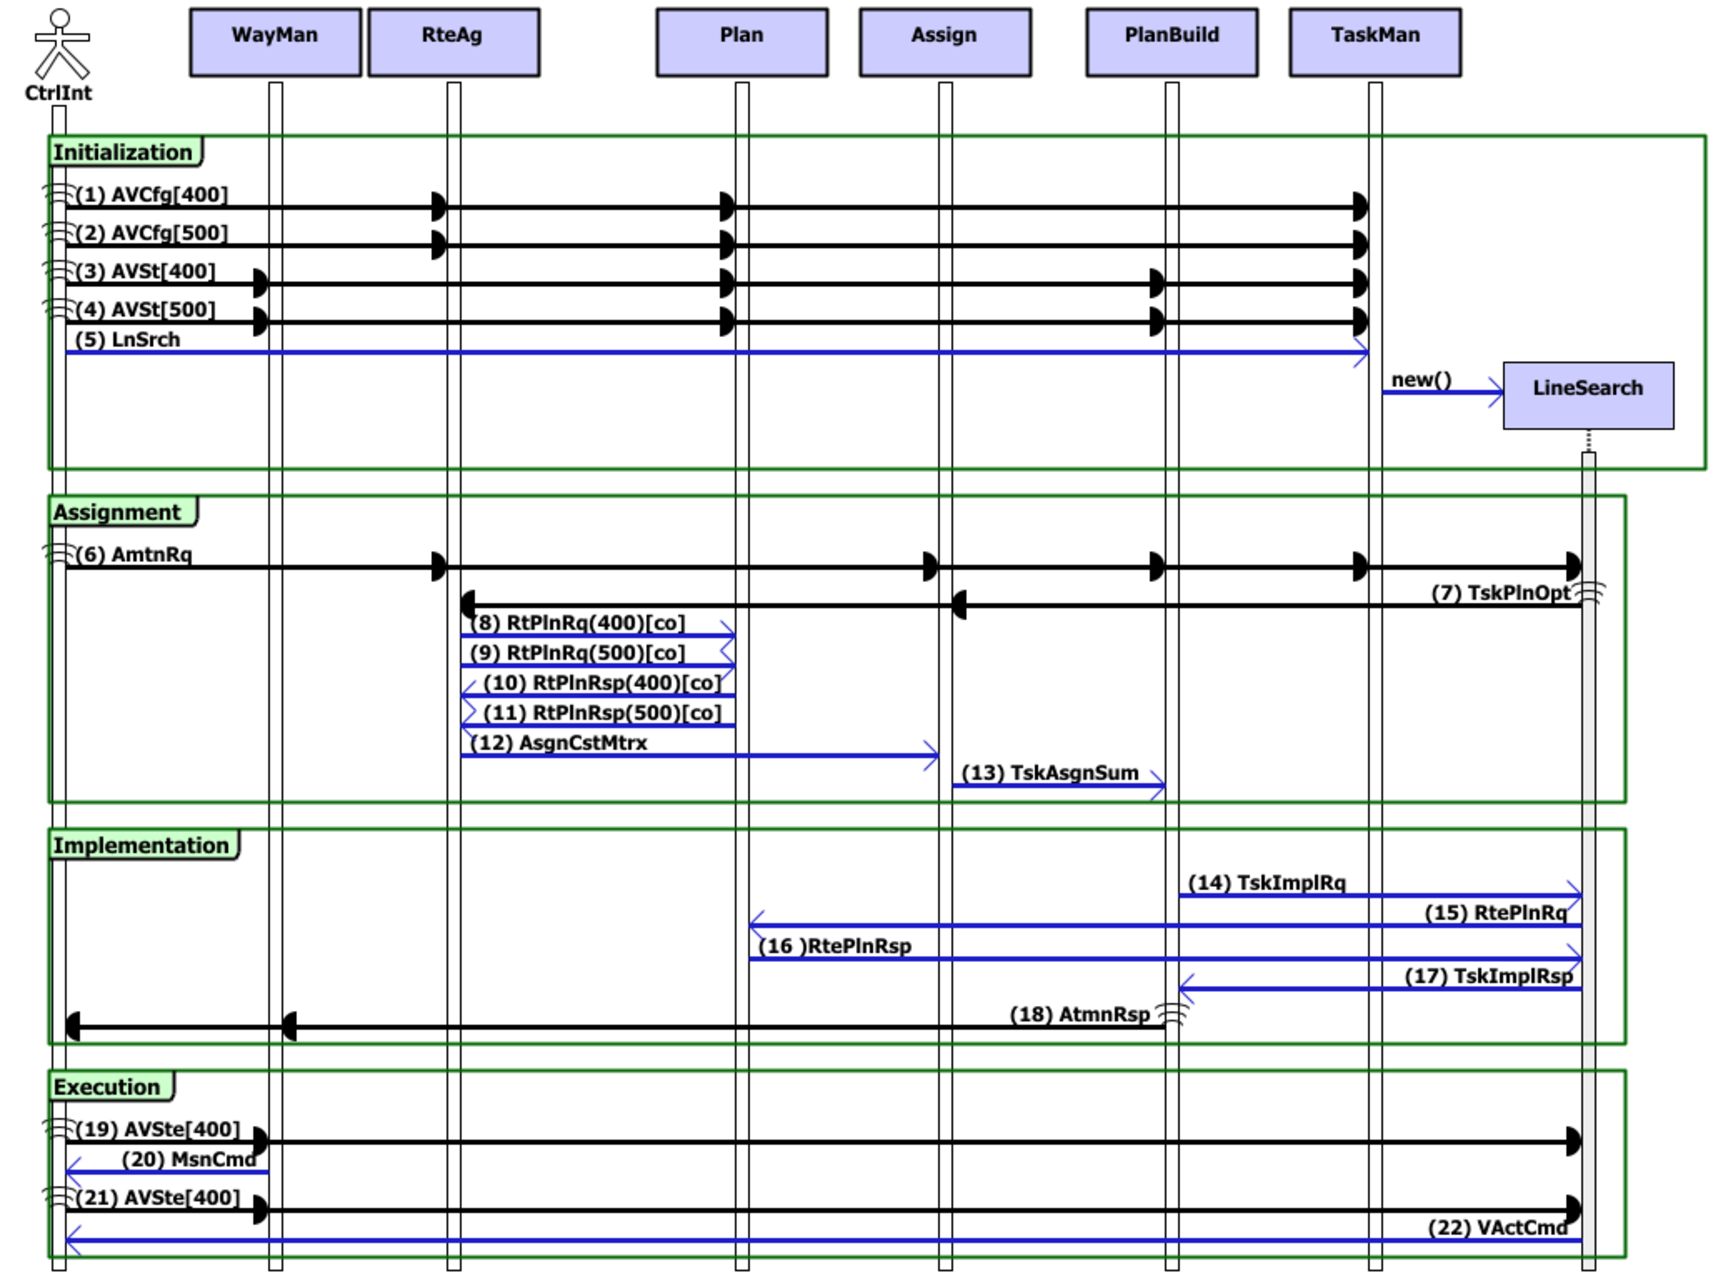
\includegraphics[width=1.3\linewidth]{\FiguresPath//WaterwaySearch_MessageFLow_Fig_all}
	\caption{The message sequence flow diagram.}
	\label{fig:MessageFlow_all}
\end{marginfigure}

\begin{itemize}
	\item The \textbf{rectangles} across the top of the diagram, and the one on the right side, represent UxAS services, which are described in the next section. 
	\item The \textbf{stick figure} labeled `CtrlInt' is the interface to a ground control station that is connected to the UAVs via radio. 
	\item The \textbf{horizontal lines} represent LMCP messages and the arrowheads show where messages are received. Note: messages are sent in order from top to bottom.
%	\item The \textbf{small rectangles} with bracketed identifiers will be used to explain actions taking place in the diagram.
\end{itemize}

\subsection{UxAS Services in the Message Flow}
\begin{description}
	\item[\textit{WayMan}] The \textbf{WaypointManager} is used during the execution phase to send small sets of waypoints to the UAVs via the ground station. It partitions the mission waypoints into overlaping sets that are small enough that they can be sent to the UAVs given communication and autopilot constraints.
	\item[\textit{RteAg}] The \textbf{RouteAggregator} perfoms two functions it manages \textit{Route Requests} and constructs the \textit{Assignment Matrix}. It receives \textbf{\textit{RouteRequest}} messages, then sends \textbf{\textit{RoutePlanRequest}} messages to an appropriate planner for the vehicle type, e.g. UAV, ground vehicle, surface ship, and then send out the resulting \textbf{\textit{RouteResponse}} messages. Once it receives \textbf{\textit{TaskOption}} messages from all of the tasks specified in the \textbf{\textit{AutomationRequest}}, it sends out the messages necessary to build a matrix of costs, \textbf{\textit{AssignmentCostMatrix}}, that is used by the \textbf{Assignment} service. 
	\item[\textit{Plan}] This \textbf{Planner} service is specialized to generate waypoints plans for a UAV to fly from a given position, with a given heading, to a second position, with a second heading. 
	\item[\textit{Assign}] The \textbf{Assignment} service minimizing a cost function uses costs generated from the \textbf{\textit{AssignmentCostMatrix}} and the \textbf{\textit{TaskOption}} messages to assign vehicles to tasks.
	\item[\textit{PlanBuild}] The \textbf{PlanBuilder} service oversees the construction of waypoint plans for the mission, based on the \textbf{\textit{TaskAssignmentSummary}}, using \textbf{\textit{TaskImplmentation}} messages to the tasks. 
	\item[\textit{TaskMan}] The \textbf{TaskManager} service receives task messages and manages creation and deletion of corresponding task services.
	\item[\textit{LinSearch}] The \textbf{LineSearchTask} service manages the functionality required to build plans to cause the UAVs to follow a given line while pointing it sensor. Note: UxAS Tasks are special services that can be instantiated by sending task messages. Tasks can be used in a persistent fashion, i.e. they can be instantiated early and then assigned many times. Each task service is responsible for constructing task implementation plans for every eligible vehicle, calculating task costs and communicating them to the other services, and commanding task activities, such as sensor pointing, during task execution.
	 
\end{description}

\subsection{Message Flow Description}
The following sections describe the message flow and how it is used to implement the Waterway Monitoring scenario. The message flow is broken into four phases: Initialization, Assignment, Implementation, and Execution. Each is described below. Note that in order to utilize the processor to best advantage, all processing is accomplished when the required information becomes available.


\newthought{Initialization}
In this phase all the information required to calculate plans and assignments is passed into UxAS via messages, see Figure \ref{fig:MessageFlow_init}.
\begin{marginfigure}
	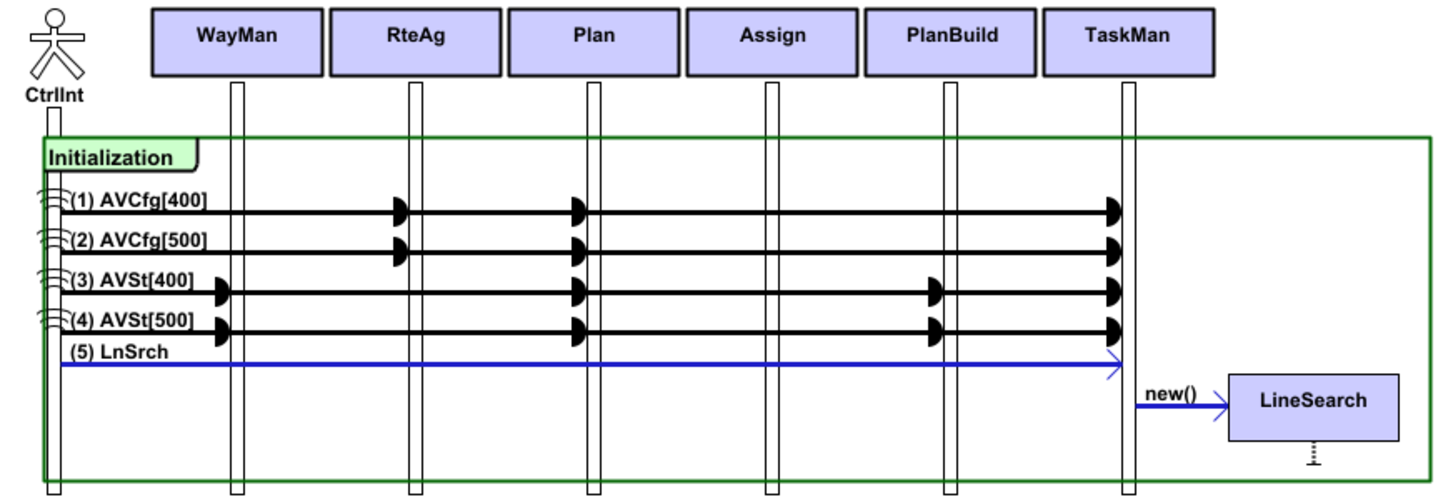
\includegraphics[width=1.3\linewidth]{\FiguresPath//WaterwaySearch_MessageFLow_Fig_init}
	\caption{The Initialization message sequence flow diagram.}
	\label{fig:MessageFlow_init}
\end{marginfigure}

\begin{marginfigure}[180pt]
	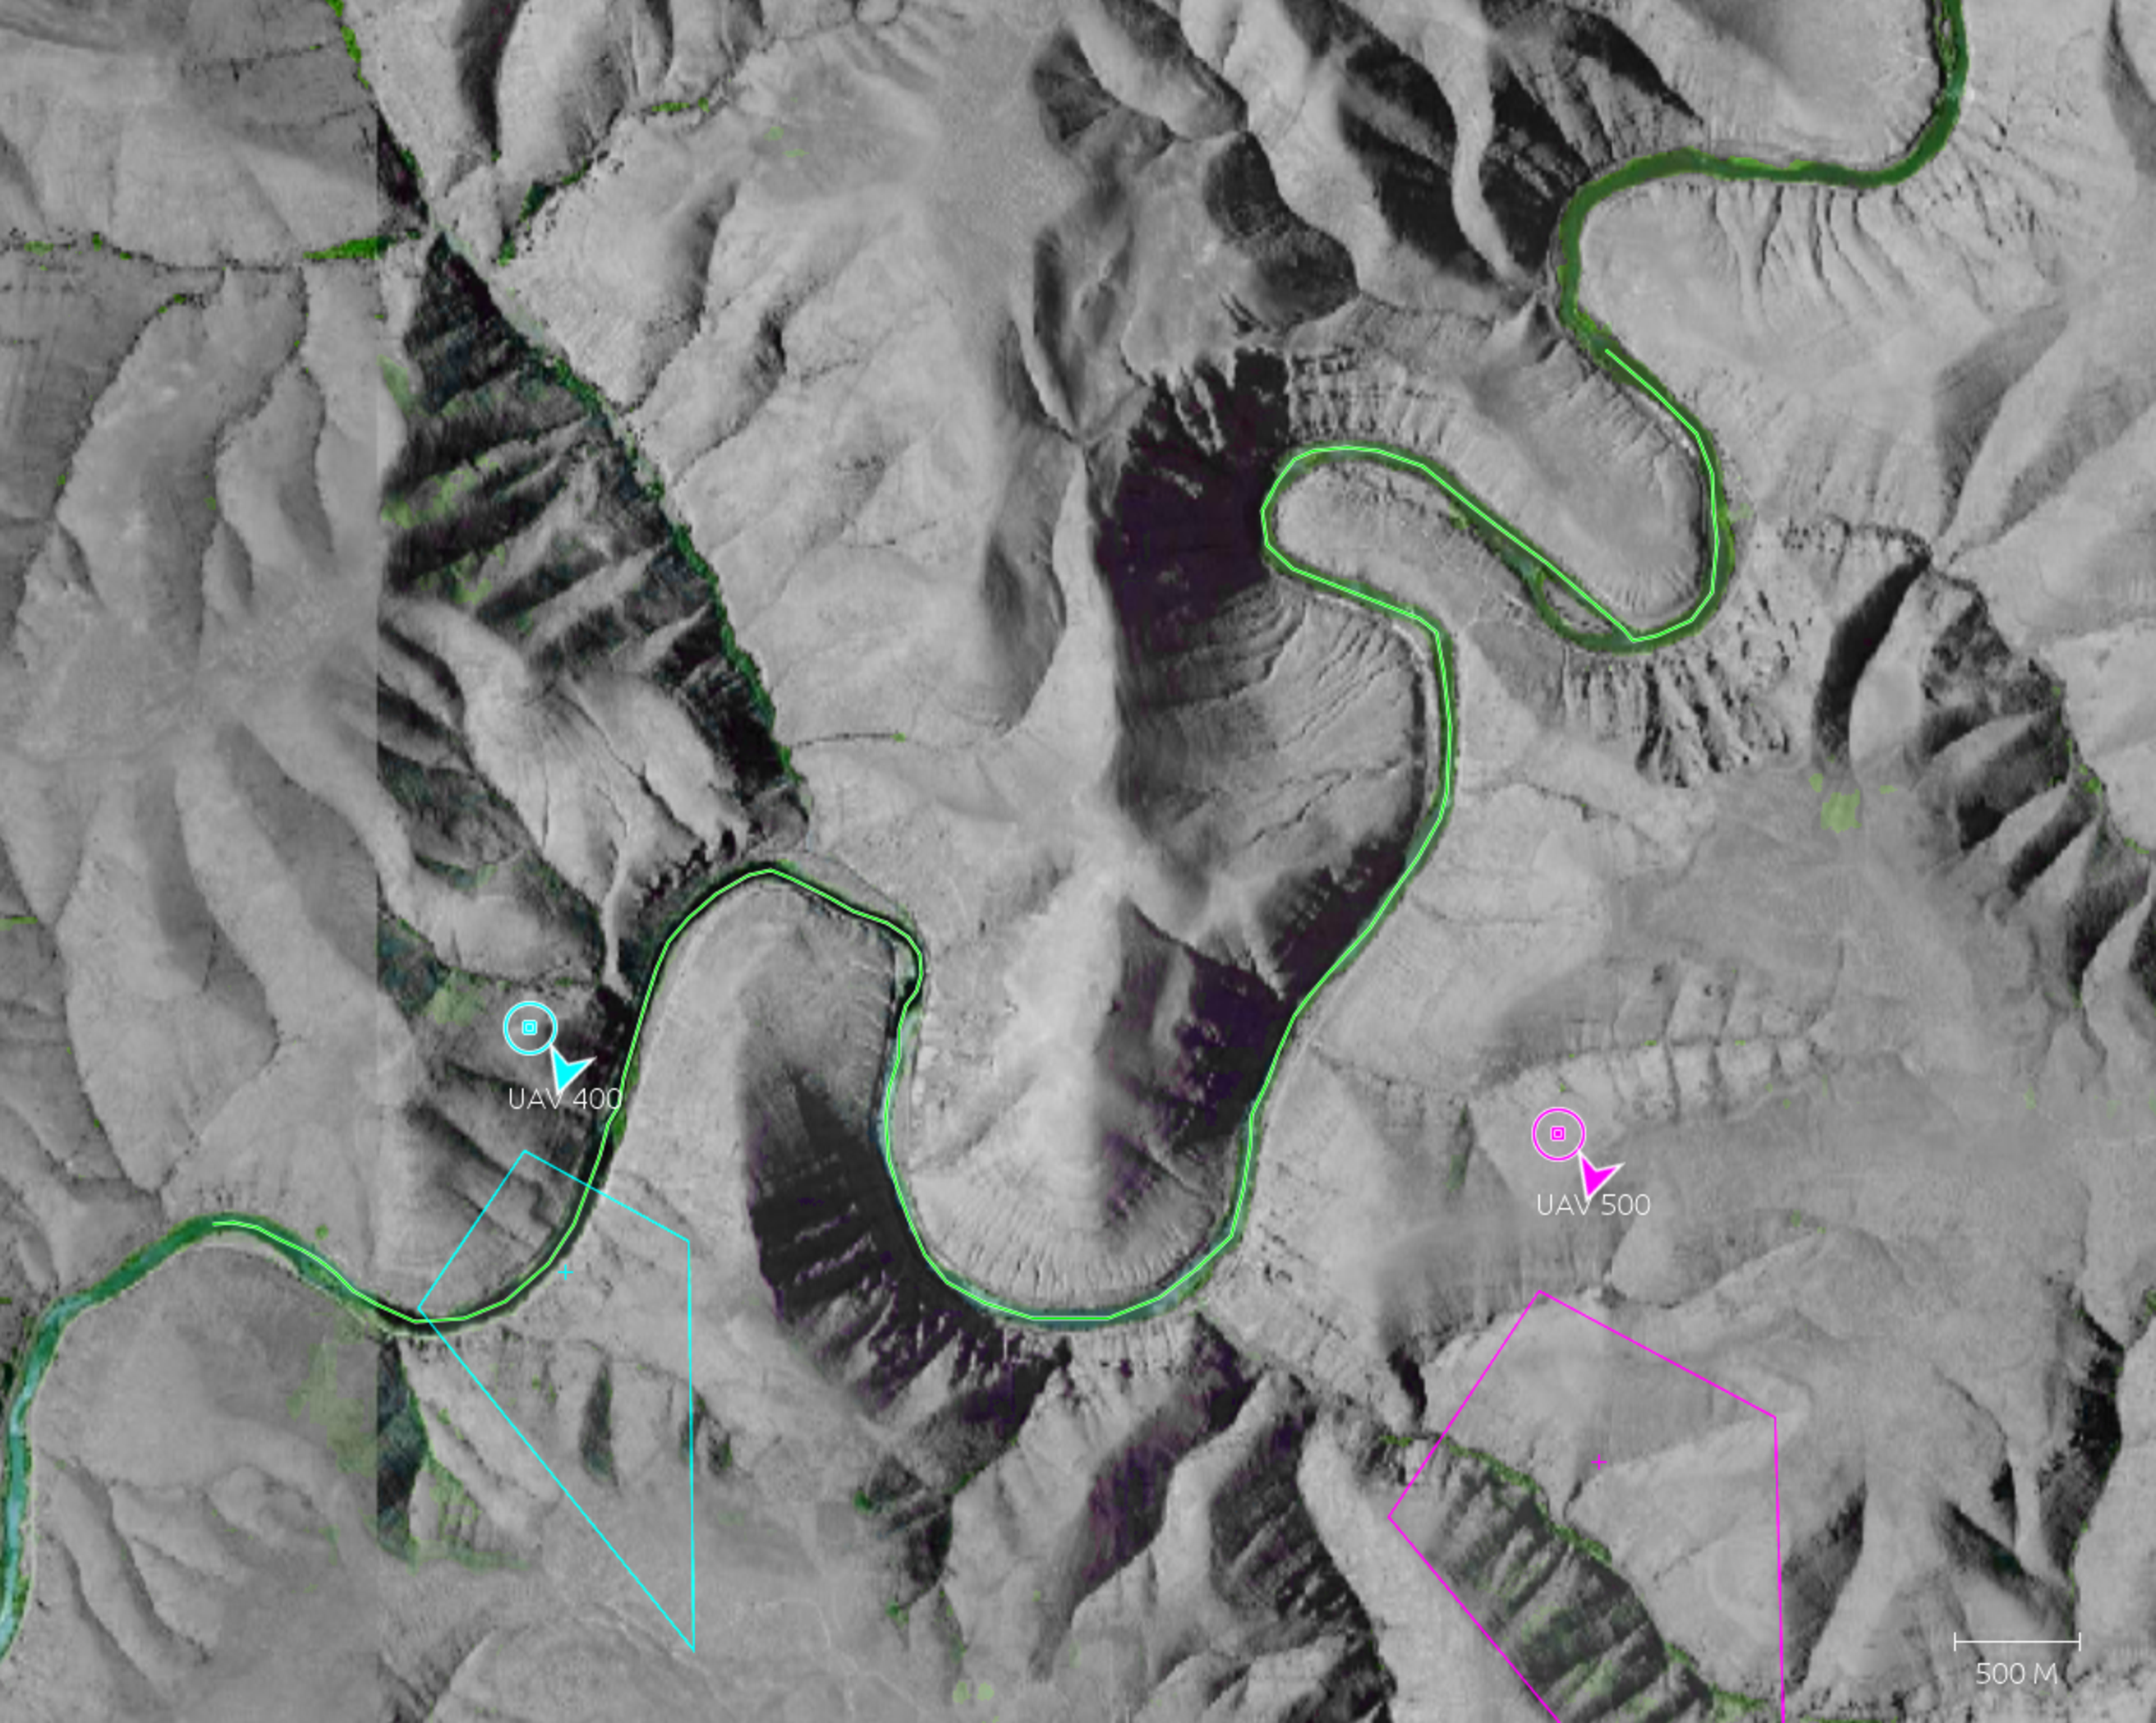
\includegraphics[width=1.3\linewidth]{\FiguresPath//02_WaterwaySearch_LineSearchTask}
	\caption{The LineSearchTask representing the waterway.}
	\label{fig:lineSearchTask}
\end{marginfigure}

\begin{description}
	\item[\hyperlink{msg:01.AirVehicleConfiguration.400}{\textbf{(1)}} and \hyperlink{msg:02.AirVehicleConfiguration.500}{\textbf{(2)}} ]  \textit{AVCfg[400]} and \textit{AVCfg[500]} are \textbf{\textit{AirVehicleConfiguration}} Messages for UAV 400 and 500, respectively. These messages are sent from the ground control station and provide UAV specific parameters used in planning and execution such as UAV operating speed, altitude, and maximum bank angle, as well as, sensor configurations.
	
	\item[\hyperlink{msg:03.AirVehicleState.400}{\textbf{(3)}} and \hyperlink{msg:04.AirVehicleState.500}{\textbf{(4)}} ]  \textit{AVSt[400]} and \textit{AVSt[500]} are \textbf{\textit{AirVehicleState}} Messages for UAV 400 and 500, respectively. These messages are sent to UxAS from the ground control station whenever the ground control station receives them from the UAVs. They provide state information from the UAVs such as, position, actual altitude, actual speed, current waypoint, current active task, and state of the sensors.

	\item[\hyperlink{msg:05.LineSearchTask}{\textbf{(5)}}] \textit{LnSrch} is a \textbf{\textit{LineSearch}} message. It defines the Waterway and defines options such as starting the search of the waterway from the given start point or permitting the search to start from either end, see Figure \ref{fig:lineSearchTask}.
	
	\item[\textbf{new()}] Based on the \textbf{\textit{LineSearch}} message, the TaskManager service send a \textbf{\textit{CreateNewService}} message to the ServiceManager, not shown, to instantiate a new \textit{LineSearch}task service. The \textbf{\textit{CreateNewService}} message contains a \textbf{\textit{XmlConfiguration}} field that the TaskManager uses to supply the new task with all existing \textbf{\textit{AirVehicleConfiguration}} and \textbf{\textit{AirVehicleState}} messages. Note: At this point the task can calculate plans for both of the UAVs, but this is delayed until they are informed of the set of candidate UAVs in the \textbf{\textit{AutomationRequest}}. 
\end{description}
\newthought{Assignment}
In this phase the costs associated with assigning UAVs to tasks are calculated and then UAV to task assignments are determined, see Figure \ref{fig:MessageFlow_assign}.
\begin{marginfigure}
	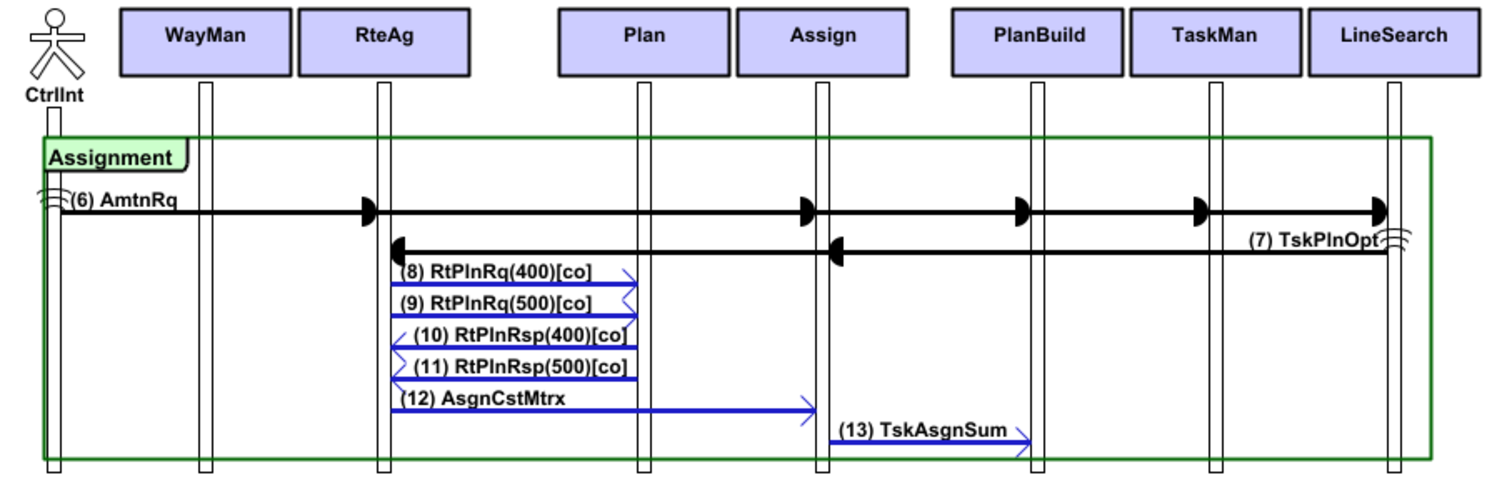
\includegraphics[width=1.3\linewidth]{\FiguresPath//WaterwaySearch_MessageFLow_Fig_assign}
	\caption{The Assignment message sequence flow diagram.}
	\label{fig:MessageFlow_assign}
\end{marginfigure}
\begin{description}
	\item[\hyperlink{msg:06.AutomationRequest}{\textbf{(6)}}]  \textit{AmtnRq} is a \textbf{\textit{AutomationRequest}} message. It is sent from the ground control station and initiates the assignment process. The \textbf{\textit{AutomationRequest}} is a \textbf{\textit{AutomationRequest}} includes IDs of the UAVs and tasks to be considered for assignment. If the ID of a task is included, the task is require to generate plans for each eligible UAVs to perform the tasks. 
	\item[\hyperlink{msg:07.TaskPlanOptions}{\textbf{(7)}}]  \textit{TskPlnOpt} is a \textbf{\textit{TaskPlanOptions}} message. Each task can have optional methods of implementation. In the waterway search example, the \textbf{\textit{LineSearchTask}} has two optional implementations, start from one end or start from the other end. Therefore the task must compute plans for each UAV to peform the task two different ways. This produces four \textbf{\textit{TaskOption}} messages and the algebra string: $(V_{1_s} or V_{1_e} or V_{2_s} or V_{2_e})$, i.e. UAV 1 performs the task starting at point $s$ or  UAV 1 performs the task starting at point $e$ or UAV 2 perform the task from either end. The \textbf{\textit{TaskOption}} messages and the algebra sting are sent out with a \textbf{\textit{TaskPlanOptions}} message.
	\item[\hyperlink{msg:08.RoutePlanRequest.400}{\textbf{(8)}}]  \textit{RtPlnRq[co]} is a \textbf{\textit{RoutPlanRequest}} (cost only) message. Once the \textbf{RouteAggregator} determines that is has received \textbf{\textit{TaskPlanOptions}} from all of the tasks contained in the \textbf{\textit{AutomationRequest}}, it constructs an assignment cost matrix by sending \textbf{\textit{RoutPlanRequest}} messages to the planner.
	\item[\hyperlink{msg:10.RoutePlanResponse.400}{\textbf{(10)}}]  \textit{RtPlnRsp[co]} is a \textbf{\textit{RoutPlanResponse}} (cost only) message. When the planner has calculated costs all of the plans in the \textbf{\textit{RoutPlanRequest}}, it returns them in a \textbf{\textit{RoutPlanResponse}} message.
	\item[\hyperlink{msg:12.AssignmentCostMatrix}{\textbf{(12)}}]  \textit{AsgnCstMtrx} is a \textbf{\textit{AssignmentCostMatrix}} message. When the route aggregator has received all required costs, it constructs and sends out the \textbf{\textit{AssignmentCostMatrix}} message.
	\item\hyperlink{msg:13.TaskAssignmentSummary}{[\textbf{(13)}}]  \textit{TskAsgnSum} is a \textbf{\textit{TaskAssignmentSummary}} message. When the \textbf{Assignment} service receives the \textbf{\textit{AssignmentCostMatrix}} message, it runs an optimization algorithm using the \textbf{\textit{AssignmentCostMatrix}} and \textbf{\textit{TaskPlanOptions}} to assign tasks to UAVs. This results in a \textbf{\textit{TaskAssignmentSummary}} message.
\end{description}



\newthought{Implementation}
During this phase waypoint plans are constructed based on the assignmnets, see Figure \ref{fig:MessageFlow_implement}.
\begin{description}
	\item[\hyperlink{msg:14.TaskImplementationRequest}{\textbf{(10)}}]  \textit{TskImplRq} is a \textbf{\textit{TaskImplementationRequest}} message. When the \textbf{PlanBuilder} service receives a \textbf{\textit{TaskAssignmentSummary}} it implements the assignments by sending \textbf{\textit{TaskImplementationRequest}} messages to the assigned tasks. It sends these requests based on the assignment order in the \textbf{\textit{TaskAssignmentSummary}}. Each task is required to construct a waypoint plan that will cause the UAV to move from its last position, and heading, to the start of the task and then append any task waypoints.
	\item[\hyperlink{msg:15.RoutePlanRequest.400}{\textbf{(15)}}]  \textit{RtePlnRq} is a \textbf{\textit{RoutePlanRequest}} message.  Tasks use the \textbf{\textit{RoutePlanRequest}} message to obtain the waypoint plans.
	\item[\hyperlink{msg:16.RoutePlanResponse.400}{\textbf{(16)}}]  \textit{RtePlnRsp} is a \textbf{\textit{RoutPlanResponse}} message. When the planner has constructed all the plans requested in the \textbf{\textit{RoutePlanRequest}} message, it send then out in a \textbf{\textit{RoutPlanResponse}} message.
	\item[\hyperlink{msg:17.TaskImplementationResponse}{\textbf{(17)}}]  \textit{TskImplRsp} is a \textbf{\textit{TaskImplementationResponse}} message. The task send back the waypoint plan in \textbf{\textit{TaskImplementationResponse}} message. Note: if there are multiple tasks assigned to a UAV, the \textbf{PlanBuilder} uses the UAV's last position and heading from the \textbf{\textit{TaskImplementationResponse}} as the starting point and heading for the next \textbf{\textit{TaskImplementationRequest}}.
	\item[\hyperlink{msg:18.AutomationResponse}{\textbf{(18)}}]  \textit{AtmnResp} is a \textbf{\textit{AutomationResponse}} message. Once the \textbf{PlanBuilder} has constructed plans for all of the task assignments, it sends them out in a \textbf{\textit{AutomationResponse}}, Figure \ref{fig:asignedWaypoints} shows the final plan to monitor the waterway.
\end{description}

\begin{marginfigure}[-600pt]
	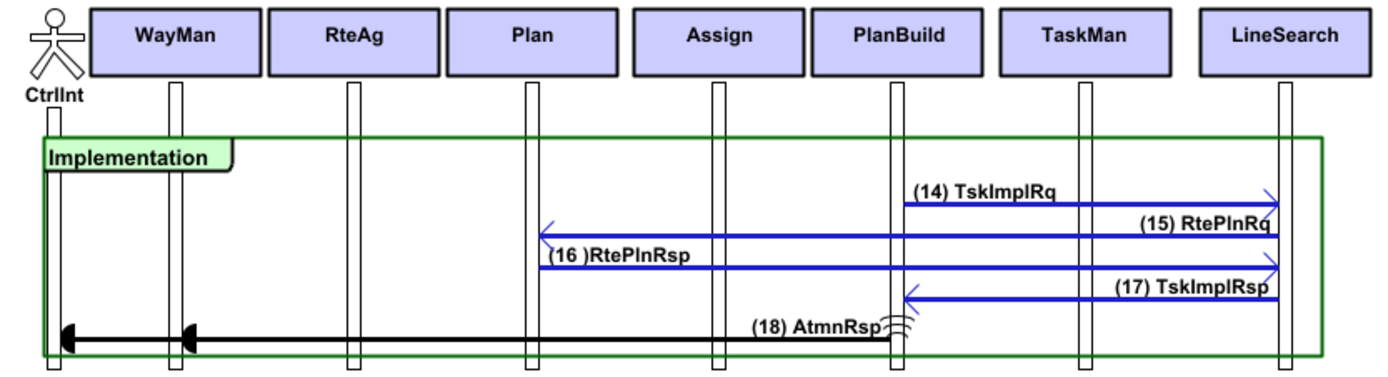
\includegraphics[width=1.3\linewidth]{\FiguresPath//WaterwaySearch_MessageFLow_Fig_implement}
	\caption{The Implementation message sequence flow diagram.}
	\label{fig:MessageFlow_implement}
\end{marginfigure}

\begin{marginfigure}[-200pt]
	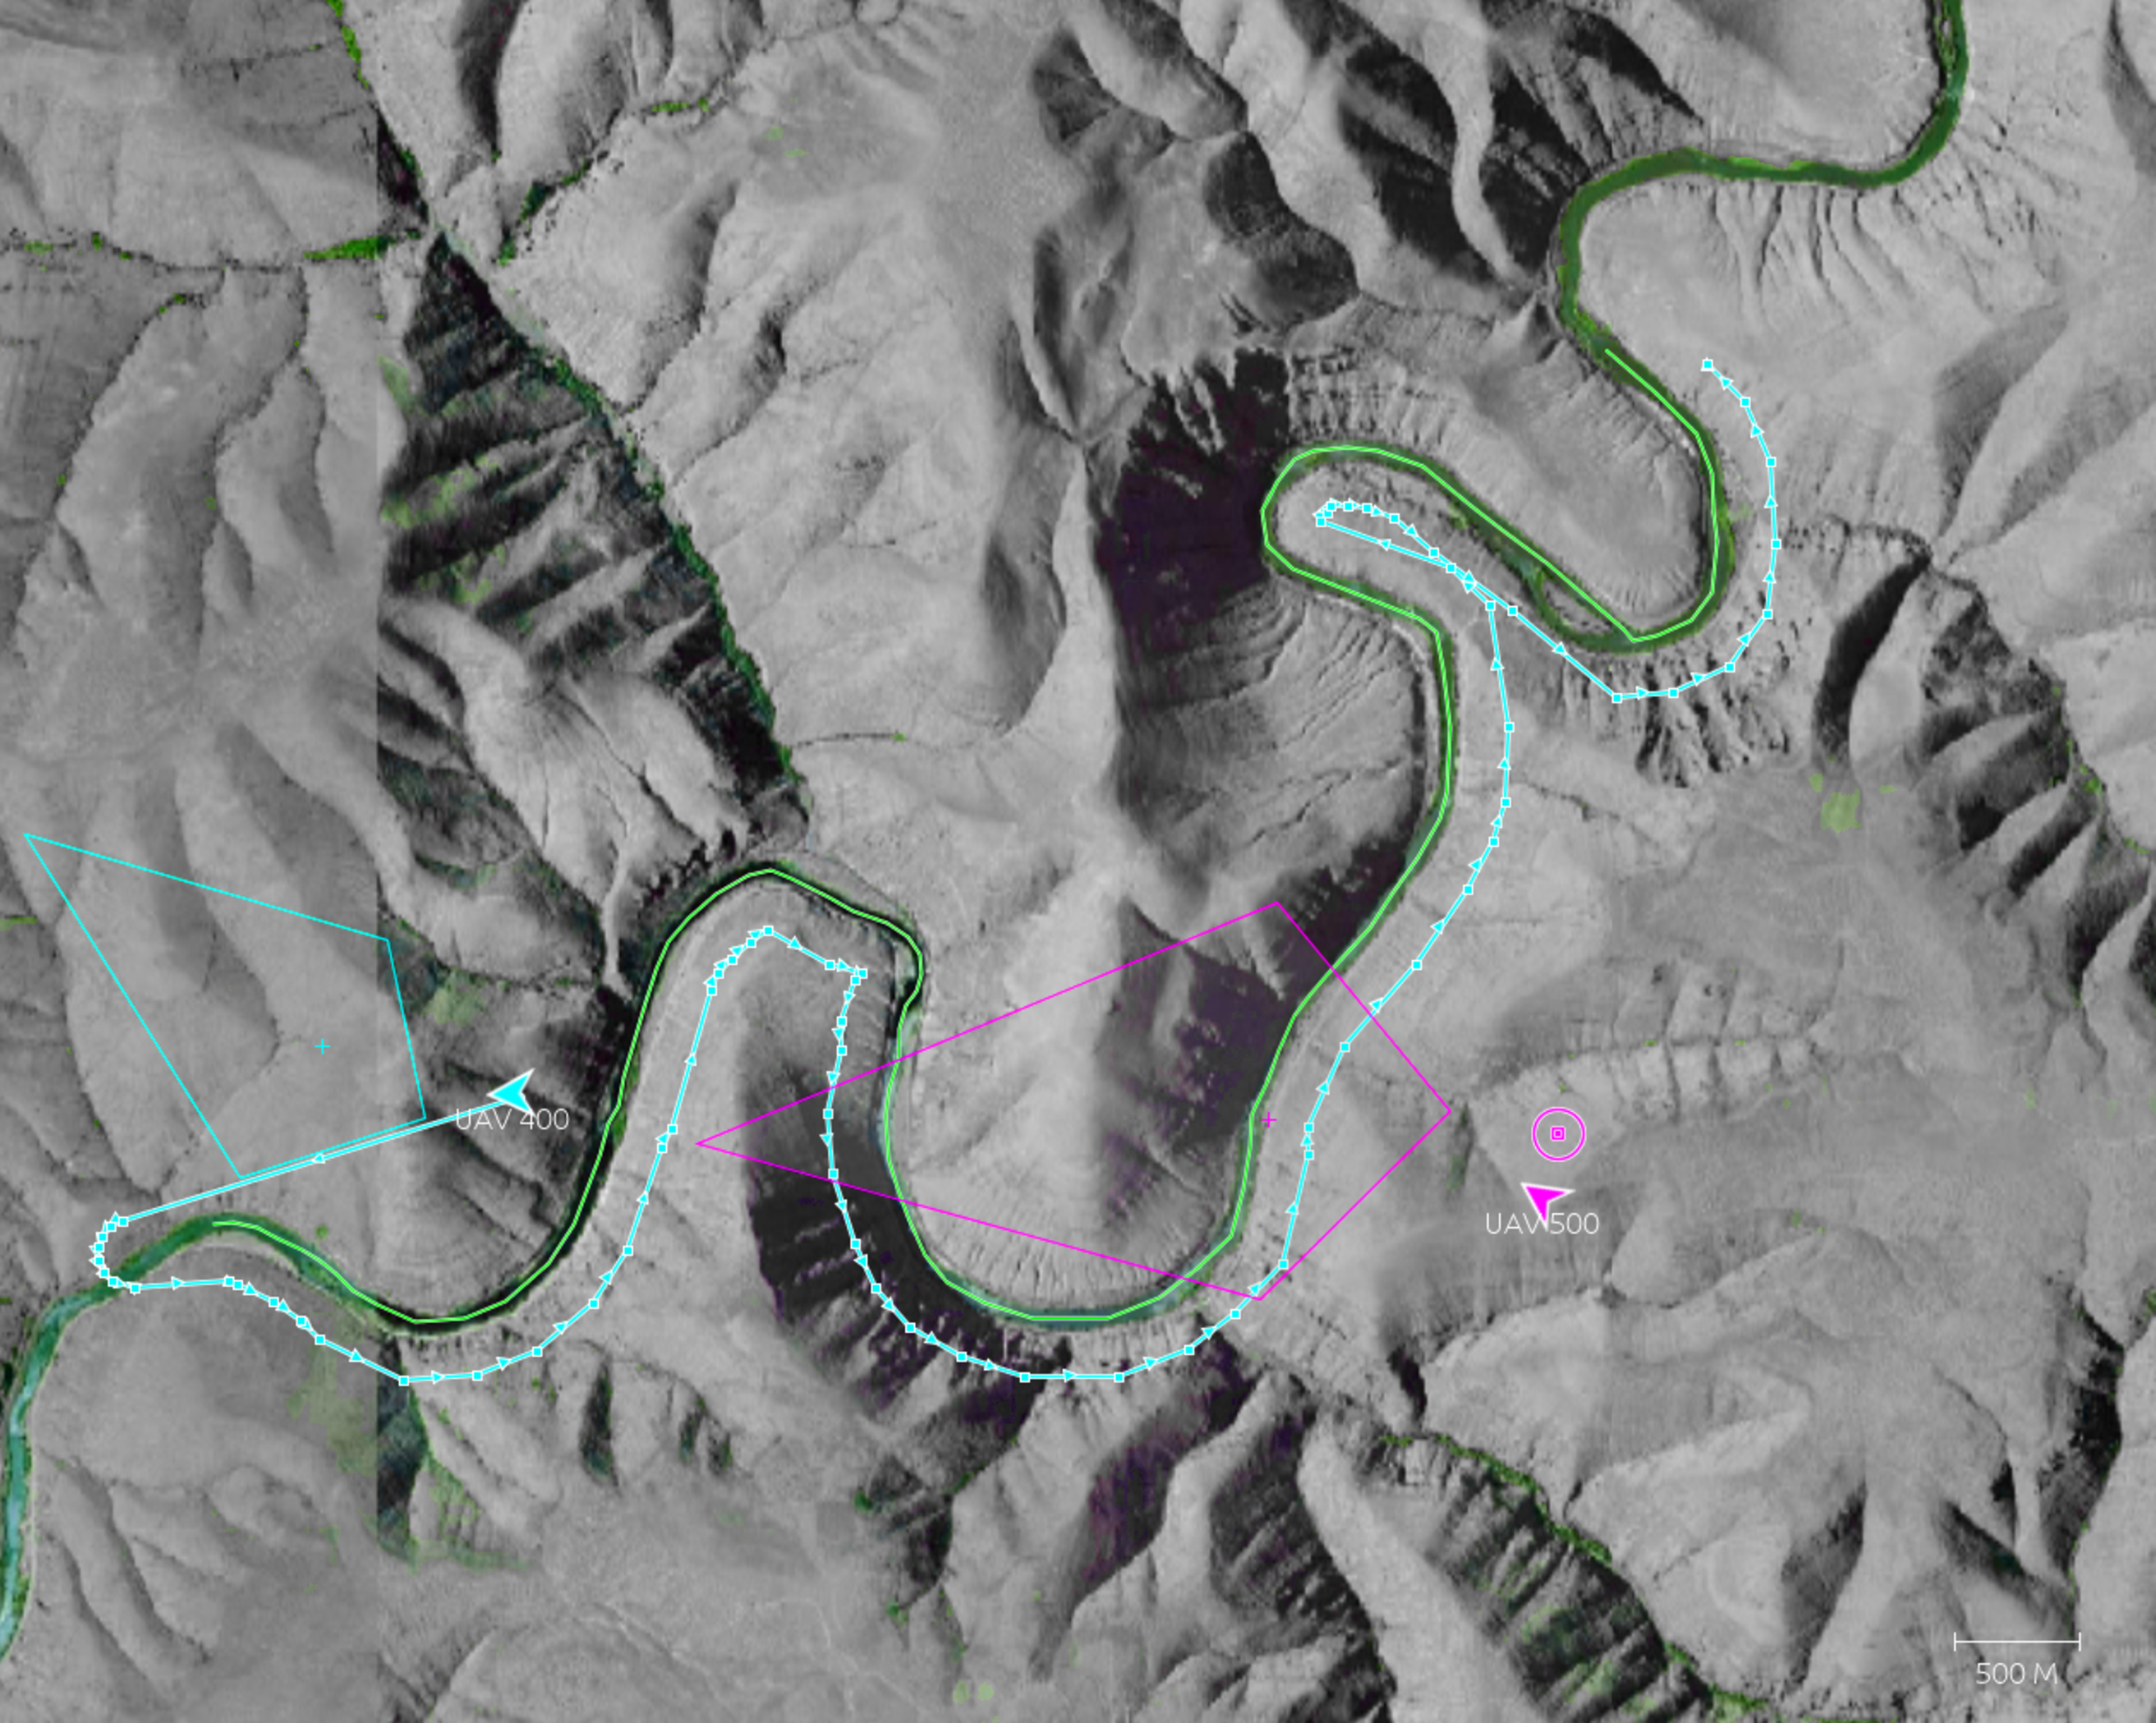
\includegraphics[width=1.3\linewidth]{\FiguresPath//03_WaterwaySearch_Assignment}
	\caption{The complete set of assigned waypoints.}
	\label{fig:asignedWaypoints}
\end{marginfigure}


\subsection{Execution}
During this phase, UxAS manages plans and, directs sensor pointing, as the plans are carried out.
\begin{marginfigure}
	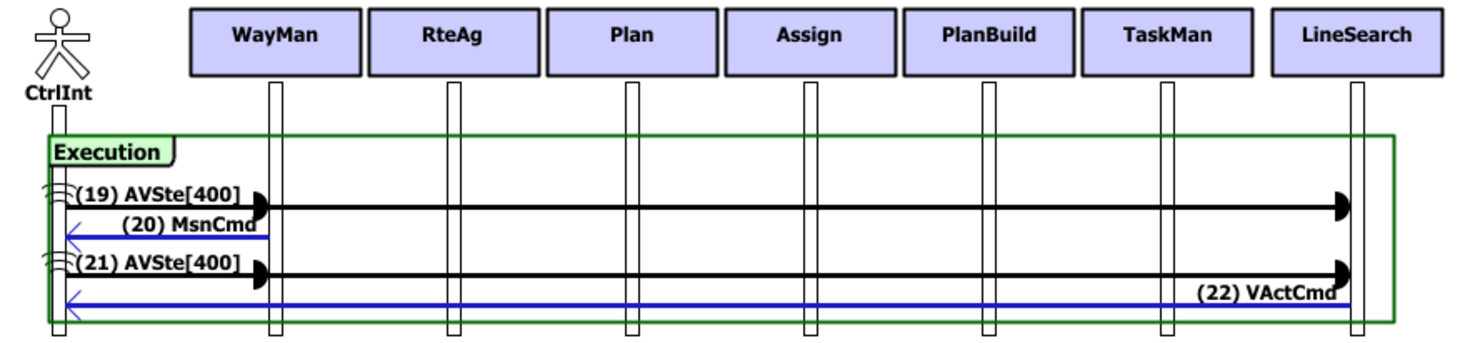
\includegraphics[width=1.3\linewidth]{\FiguresPath//WaterwaySearch_MessageFLow_Fig_execute}
	\caption{The Execution message sequence flow diagram.}
	\label{fig:MessageFlow_execute}
\end{marginfigure}

\begin{marginfigure}
	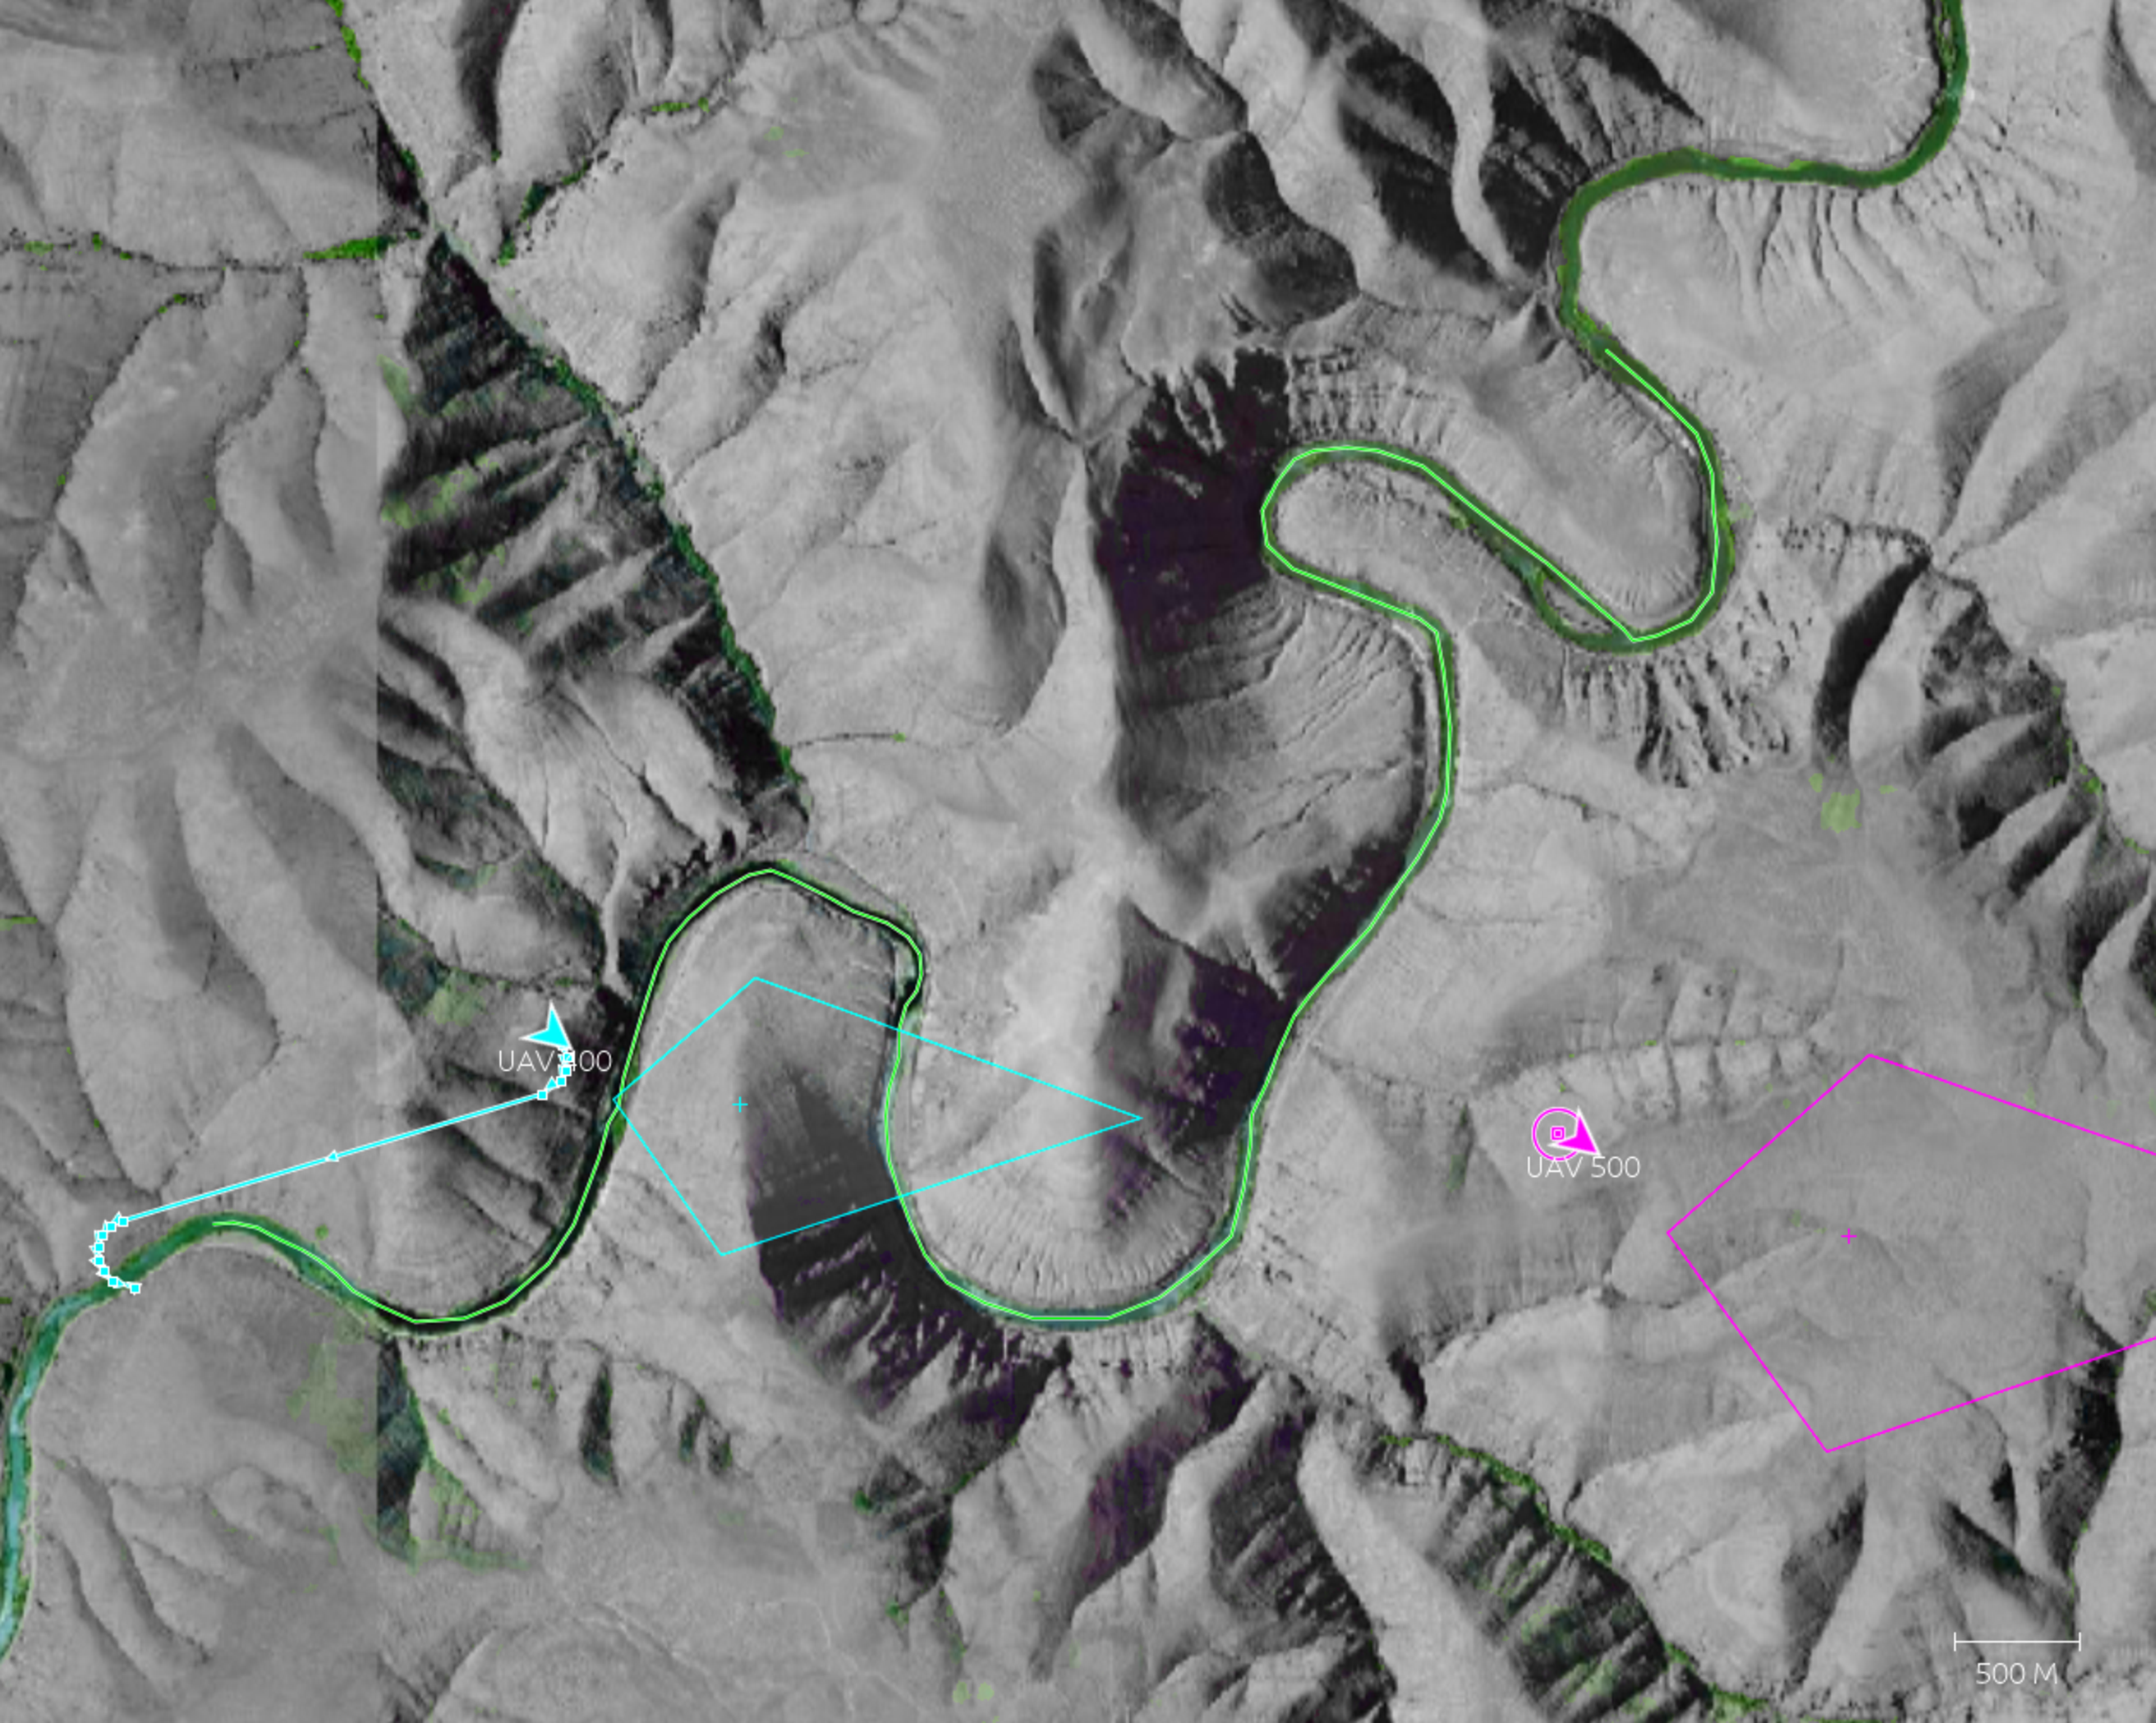
\includegraphics[width=1.3\linewidth]{\FiguresPath//04_WaterwaySearch_BeginExecution}
	\caption{Start executing the plan.}
	\label{fig:startExecution}
\end{marginfigure}

\begin{description}
	\item[\hyperlink{msg:19.AirVehicleState.400}{\textbf{(19)}}]  \textit{AVSt[400]} is a \textbf{\textit{AirVehicleState}} message, from UAV 400. The UAV reports its state to the ground control station which, in turn, send a \textbf{\textit{AirVehicleState}} message to UxAS. 
	\item[\hyperlink{msg:20.MissionCommand.400}{\textbf{(20)}}]  \textit{MsnCmd} is a \textbf{\textit{MissionCommand}} message. When the \textbf{MissionManager} receives an \textbf{\textit{AirVehicleState}} message it determines which small set of waypoints the UAV is flying. If the UAV is a given number of waypoints from the end of the small set, the WaypointManager sends out the next small set of waypoints in a \textbf{\textit{MissionCommand}} message, see Figure \ref{fig:startExecution}.
	\item[\hyperlink{msg:21.AirVehicleState.400}{\textbf{(21)}}]  \textit{AVSt[400]} is a \textbf{\textit{AirVehicleState}} message, from UAV 400. The UAV reports its state to the ground control station which, in turn, send a \textbf{\textit{AirVehicleState}} message to UxAS. 
	\item[\hyperlink{msg:22.VehicleActionCommand.400}{\textbf{(22)}}]  \textit{VActCmd} is a \textbf{\textit{VehicleActionCommand}} message that implements a \textbf{\textit{GimbalStareAction}}. The task is responsible for sending any messages necessary to implement its functionality during the execution phase. When a task receives an \textbf{\textit{AirVehicleState}} message it checks the \textit{AssociatedTasks} list for its ID. If the task's ID is contained in the \textit{AssociatedTasks} list, the task is \textit{active} and, in this example, based on the UAV's position, calculates a location on the waterway to point the sensor. The UAV is commanded to point the sensor using the  \textbf{\textit{GimbalStareAction}} message, see Figure \ref{fig:pointGimbal}.  
\end{description}

\begin{marginfigure}
	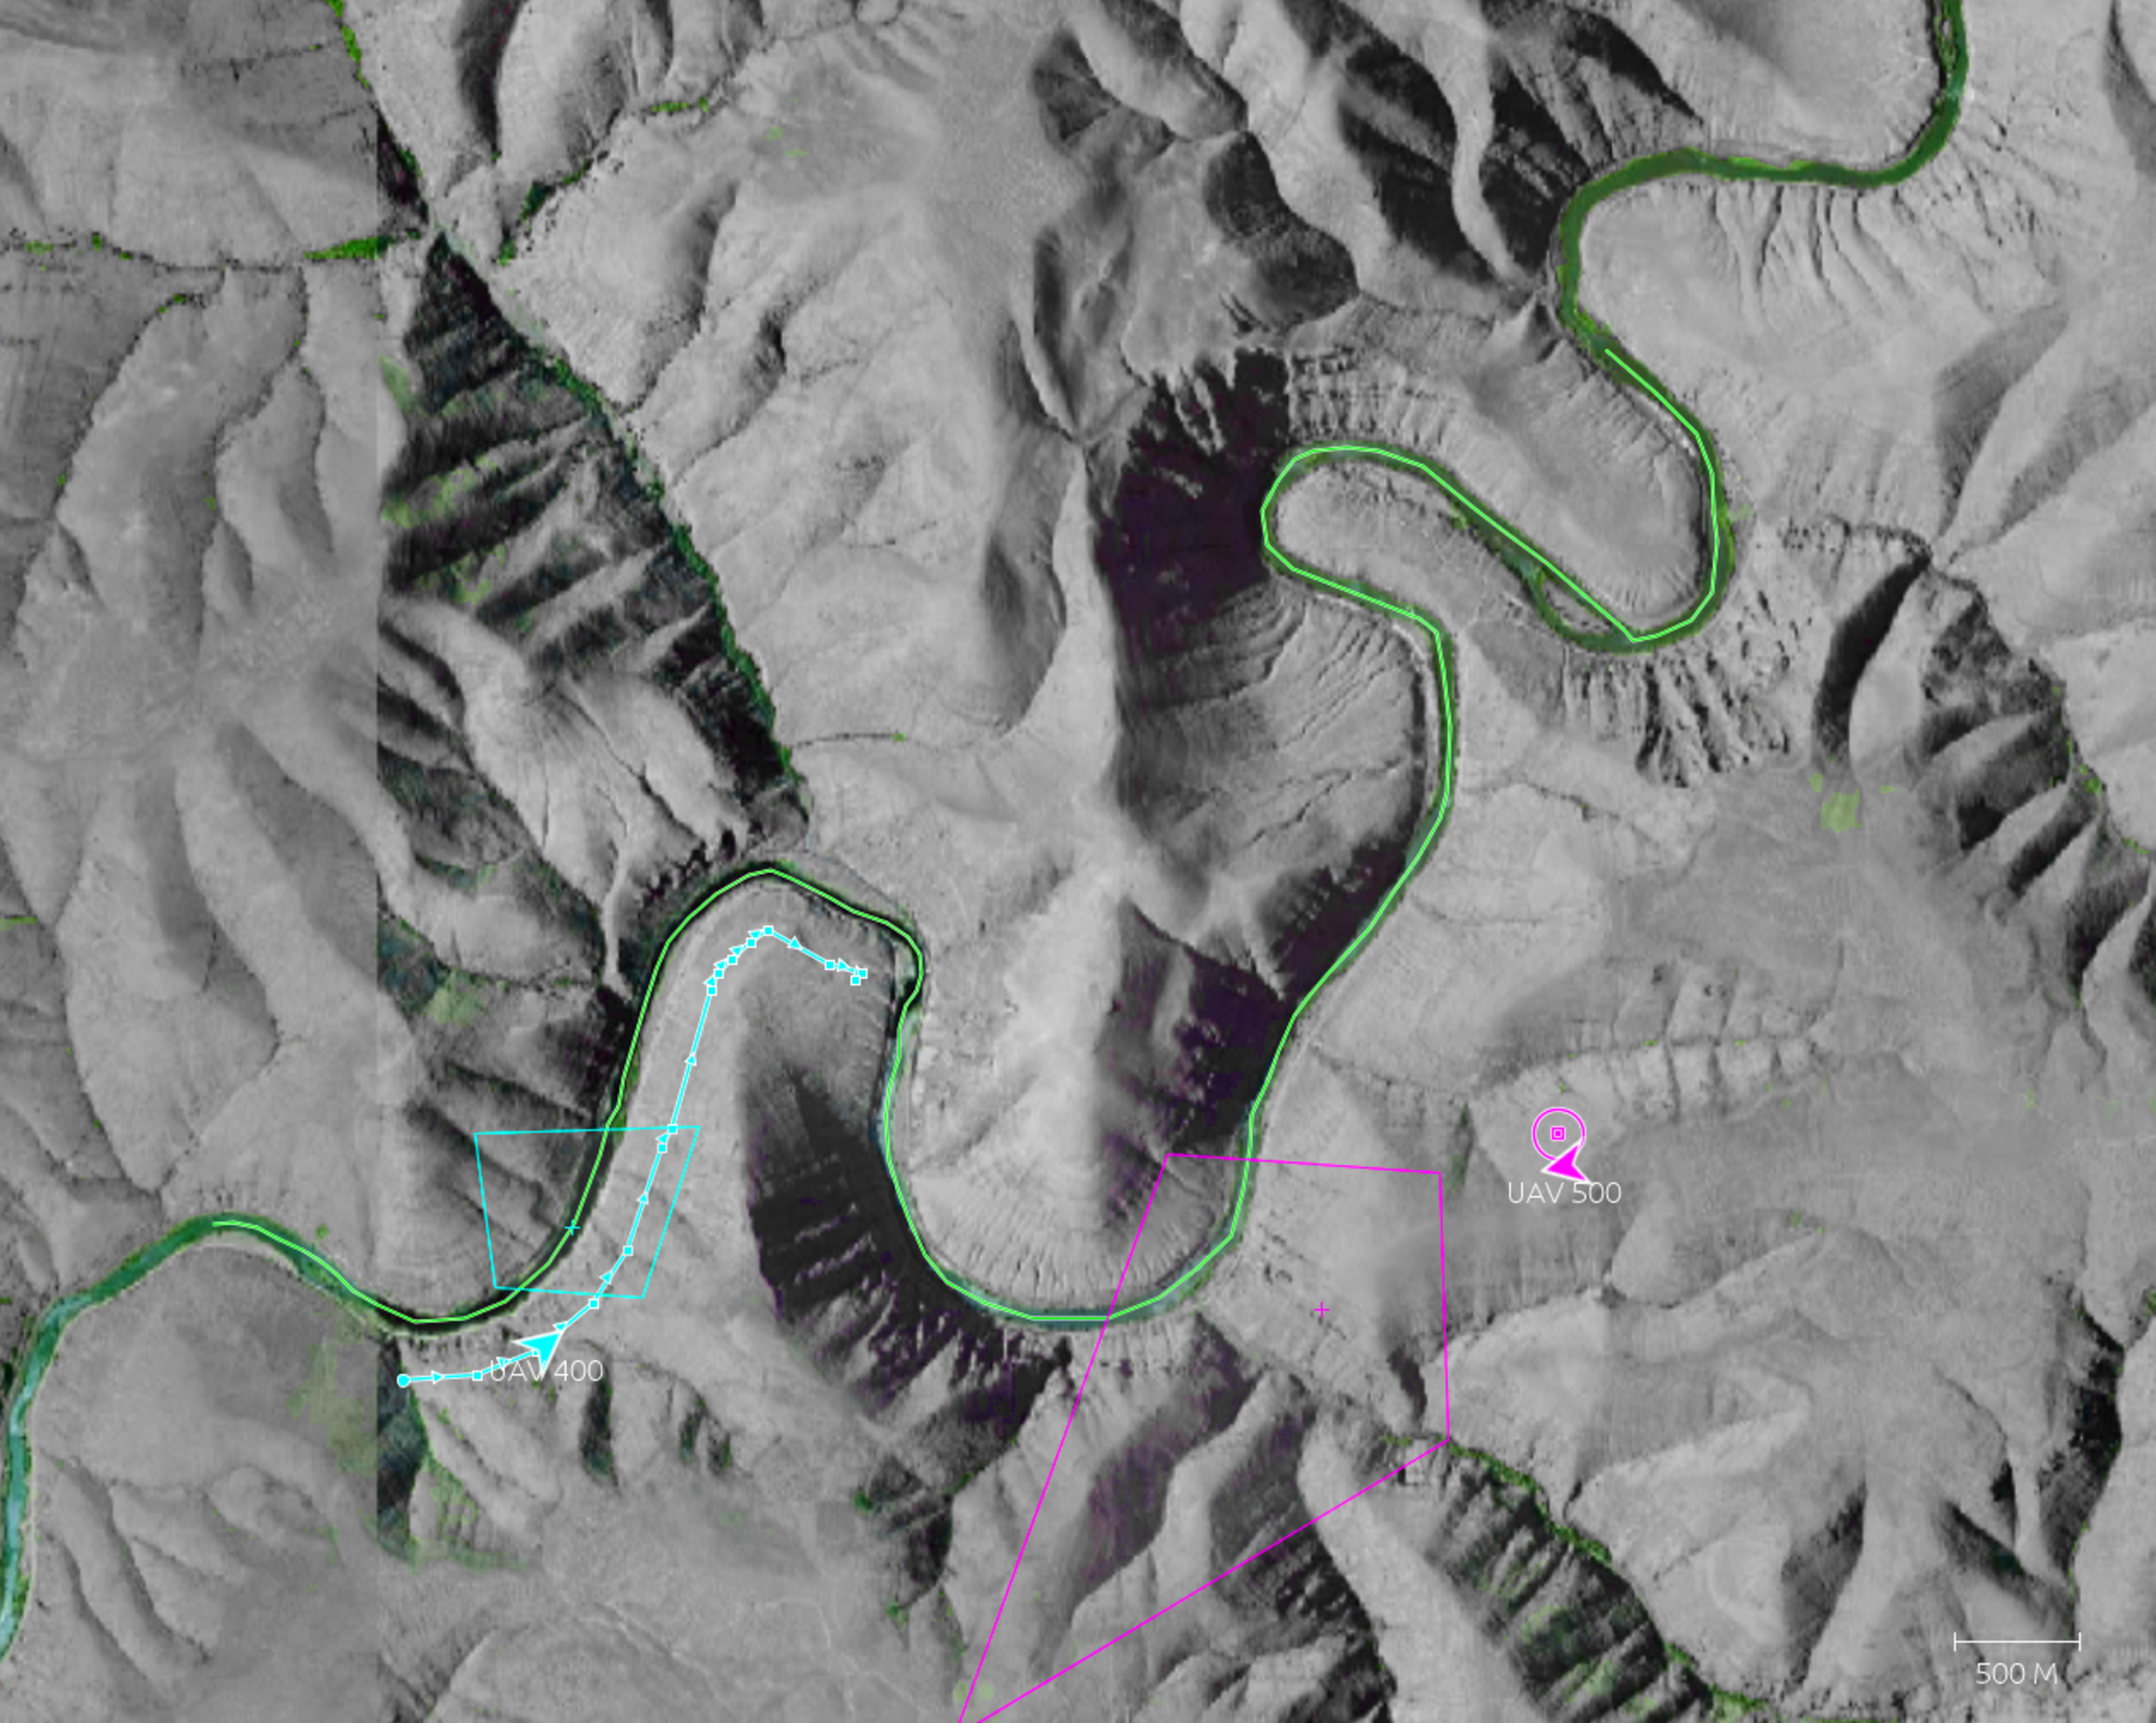
\includegraphics[width=1.3\linewidth]{\FiguresPath//05_WaterwaySearch_PointSensor}
	\caption{Pointing the sensor along the waterway.}
	\label{fig:pointGimbal}
\end{marginfigure}
